%!TeX root=main.tex
\chapter{مروری بر کار‌های مرتبط}
\thispagestyle{empty}

در سال‌های اخیر تحقیقات در تشخیص موضع افزایش چشم‌گیری داشته است (شکل~\ref{StancePublicationPerYear}). در این بخش ابتدا رقابت‌های برگزار شده در زمینه تشخیص موضع را مورد بررسی قرار می‌دهیم. سپس تعدادی از مجموعه دادە‌های معرفی شده را بررسی می‌کنیم. در ادامه رویکردهای معرفی شده برای تشخیص موضع را معرفی می‌کنیم.

\begin{figure}[H]
	\center{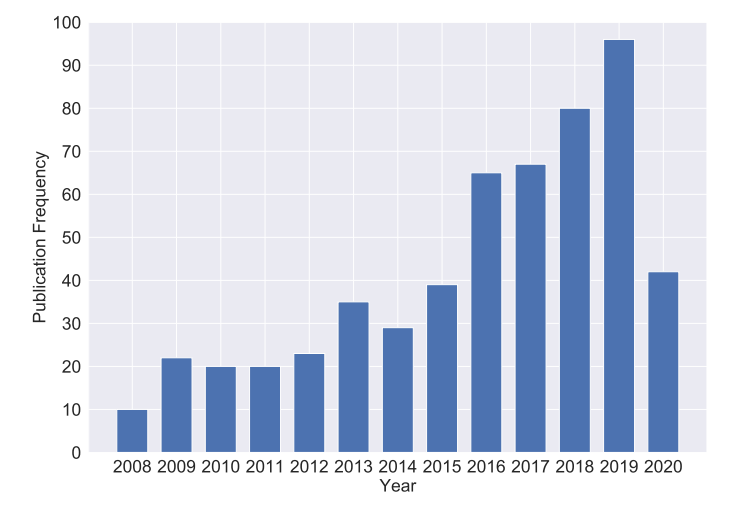
\includegraphics[width=0.7\linewidth]{images/StancePublicationPerYear.PNG}}
	\caption[نمودار تعداد مقالات چاپ شده در رابطه با تشخیص موضع به تفکیک سال]
	{نمودار تعداد مقالات چاپ شده در رابطه با تشخیص موضع به تفکیک سال. جستجو براساس
		کلمات کلیدی «تشخیص موضع»، «پیش بینی موضع» و «ردە‌بندی موضع» انجام شده است \cite{ALDAYEL2021102597}.}

	\label{StancePublicationPerYear}
\end{figure}

\section{رقابت‌های برگزار شده در مسئله تشخیص موضع}
با بررسی منابع موجود، مشخص شد تا کنون شش رقابت در رابطه با مسئله تشخیص موضع برگزار شده است. در این رقابت‌ها مجموعە دادە‌های جدید و مدل‌های مرتبط با آن‌ها معرفی می‌شوند. بنابراین برگزاری چنین رویدادهایی نقش مهمی در رشد و تقویت تحقیقات در تشخیص موضع دارند \cite{10.1145/3369026}. مهم‌ترین رویدادهای برگزار شده به شرح زیر است.
\subsection{رویداد
	\lr{SemEval-2016}}
اولین رقابت برگزار شده برای مسئله تشخیص موضع، رقابت 
\href{https://alt.qcri.org/semeval2016/task6/}{\lr{SEMEval2016:Task6}}\LTRfootnote{\href{{https://alt.qcri.org/semeval2016/task6/}}{{https://alt.qcri.org/semeval2016/task6/}}}
می‌باشد. در این رقابت چندین مسئله تعریف شده که مسئله ششم مرتبط با تشخیص موضع می‌باشد. این رقابت شامل دو زیر مسئله است \cite{mohammad-etal-2016-semeval}.

\begin{enumerate}
	\item تشخیص موضع با نظارت
	\LTRfootnote{\lr{Supervised Stance Detection}}
	\newline
	مجوعه داده دارای برچسب برای ۵ موضوع
	\LTRfootnote{\lr{Target}}
	 که دارای ۲۸۱۴ توییت در قسمت دادە‌های آموزشی و
	۱۲۴۹ توییت در دادە‌های ارزیابی می‌باشد.
	\item تشخیص موضع با نظارت ضعیف
	\LTRfootnote{\lr{Weakly Supervised Stance Detection}}
	\newline
	شامل حدودا ۷۸۰۰۰ توییت بدون برچسب به عنوان دادە‌های آموزشی می‌باشد. دادە‌های ارزیابی شامل ۷۰۷ توییت در رابطه با هدف دیگری می‌‌باشد.
\end{enumerate}

	در مجموع ۱۹ گروه در این رقابت شرکت کردند. شرکت کنندگان در این مسابقه از روش‌های مختلفی استفاده کردند. روش‌های استفاده شده شامل یادگیری ماشین سنتی مبتنی بر ویژگی
	\LTRfootnote{\lr{Feature-Based Machine Learning}}
	، یادگیری عمیق و یادگیری مجمع
	\LTRfootnote{\lr{Ensemble Learning}}
	می‌باشد. بهترین مدل معرفی شده برای زیر مسئله اول (تشخیص موضع با نظارت)، از	یادگیری مجمع شبکه عصبی بازگشتی 
	\lr{(RNN)} 
استفاده کرده است. در ارزیابی نهایی، این روش به مقدار
\lr{67.82\%}
برای معیار
\lr{F1-Score}
دست یافت \cite{zarrella-marsh-2016-mitre}. همچنین بهترین مدل (در قیاس با ۹ روش معرفی شده) برای زیر مسئله دوم (تشخیص موضع با نظارت ضعیف) از شبکه عصبی پیچشی 
\lr{(CNN)}
استفاده کرد که در ارزیابی پایانی مقدار
 \lr{56.28\%}
 برای معیار
 \lr{F1-Score}
 دست یافت \cite{wei-etal-2016-pkudblab}. علاوه بر این، مدل مبتنی بر شبکه عصبی پیچشی
 \lr{(CNN)}
 با مقدار
  \lr{67.33\%}
  برای معیار
   \lr{F1-Score}
جایگاه دوم را برای زیر مسئله اول کسب کرد. مدل پایە‌ای که توسط طراحان مسابقه توسعه یافته از روش 
\lr{SVM}
استفاده کرده است. در ارزیابی انتهایی به مقدار
 \lr{68.98\%}
 برای معیار
\lr{F1-Score}
دست یافت. این بالاترین مقدار در بین همه شرکت کنندگان در رویداد می‌باشد.
 
%\iffalse
\subsection{رویداد
	\lr{NLPCC-ICCPOL-2016}}

رقابت
\lr{NLPCC-ICCPOL-2016}
تشخیص موضع بر روی وبلاگ‌های کوتاه به زبان چینی است \cite{10.1007/978-3-319-50496-4_85}. در این
رقابت چندین مسئله تعریف شده که مسئله چهارم مرتبط با تشخیص موضع می‌باشد. در این رقابت نیز دو زیر مسئله مشابه با
\lr{SemEval-2016}
 تعریف شد.
 
 \begin{enumerate}
 	\item تشخیص موضع با نظارت
 	
 	حدود ۴۰۰۰ وبلاگ کوتاه به صورت دستی
 		\LTRfootnote{\lr{Manual}}
 	 برای ۵ موضوع حاشیە نویسی شده است. موضوعات
 	شامل
 	 \lr{SE iPhone}،
 	  ترقی در جشنواره بهار، عملیات ضد تروریستی روسیه در سوریه، سیاست دو فرزند و ممنوعیت موتورسیکلت و محدودیت وسایل نقلیه الکترونیکی در شنژن می‌باشد. از این میان
 	\lr{75\%}
 	 دادە‌ها برای آموزش و مابقی دادە‌ها برای ارزیابی استفاده می‌شوند.
 	
 	\item 
 	تشخیص موضع بدون ناظر
	\LTRfootnote{\lr{Unsupervised Stance Detection}}
	
	در این روش از مجموعه داده بدون برچسب برای آموزش بدون ناظر استفاده می‌شود. دادە‌های این قسمت شامل ۲۴۰۰ وبلاگ کوتاه بدون برچسب است. این دادە‌ها شامل دو موضوع موارد غذایی اصلاح شده ژنتیکی و آزمایش‌های هستە‌ای کره شمالی می‌باشند.
 \end{enumerate}

در این رقابت شانزده تیم در زیر مسئله اول (تشخیص موضع با نظارت) و پنج تیم در زیر مسئله دوم (تشخیص موضع بدون ناظر) شرکت کردند. برنده رقابت در زیر مسئله اول، یک مدل ردە بندی جداگانه برای
هر موضوع آموزش داده است. پایه مدل‌های استفاده شده 
\lr{SVM}
 و 
 \lr{Forest Random}
  هستند. بالاترین مقدار
  \lr{F1-Score}
 به دست آمده برابر با
 \lr{71.06\%}
 می‌باشد.
 
 ویژگی‌های ورودی بهترین سیستم شامل
 \lr{Unigram}،
 \lr{TF-IDF}	\LTRfootnote{\lr{Term Frequency-Inverse Document Frequency}}،
  کلمات مشابه و بردارهای بازنمایی در سطح کلمه و کاراکتر می‌‌باشد. سایر ویژگی‌های استفاده شده توسط سایر شرکت کنندگان شامل 
  \lr{Bigram}
   و واژگان شامل احساسات 
\LTRfootnote{\lr{Sentiment Lexicons}}
   می‌باشد. همچنین با بررسی نتایج شرکت کنندگان این نتیجه حاصل شد که نتیجه بهتر در مسئله تحلیل احساسات لزوما به این معنا نیست که مدل می‌تواند در مسئله تشخیص موضع نیز به نتایج خوبی دست پیدا کند. بالاترین نتیجه کسب شده برای زیر مسئله دوم (تشخیص موضع بدون ناظر) برابر با
    \lr{46.87\%} 
    است.
\subsection{رویداد
	\lr{IberEval-2017}}

رویداد
\lr{IberEval-2017}
مشابه با دو رویداد قبلی می‌باشد. یکی از مسائل تعریف شده در این رقابت مربوط به تشخیص موضع و تشخیص جنسیت در زبان اسپانیایی و کاتالان می‌باشد \cite{taule2017overview}.

روش‌های متداول استفاده شده توسط شرکت کنندگان شامل
\lr{SVM}
، شبکه عصبی، روش‌های یادگیری
عمیق از جمله 
\lr{LSTM}
 می‌باشد. همچنین ویژگی‌های
 \lr{ngram}
  و بازنمایی کلمات
  	\LTRfootnote{\lr{word embedding}}
   از جمله متداول‌ترین ویژگی‌های استفاده شده برای این مسئله بود.
   
   ده تیم در این رقابت شرکت کردند. بهترین مدل معرفی شده برای تشخیص موضع در زبان اسپانیایی روش
    \lr{SVM}
     با ترکیبی از چندین ویژگی مطرح شده در قسمت بالا به عنوان ورودی مدل است. این در حالی است که مدل 
     \lr{Logistic Regression}
     برای زبان کاتالان به نتیجه بهتری دست یافته است. روش‌های یادگیری عمیق نتایج خوبی در این رقابت کسب نکردە اند.
   
\subsection{رویداد
	\lr{SadriStance@EVALITA-2020}}
رویداد  
\lr{SadriStance@EVALITA-2020}
اولین رقابت برگزار شده در تشخیص موضع به زبان ایتالیایی می‌باشد.
مجموعه داده جمع‌آوری‌شده درباره موضوع جنبش
\href{https://en.wikipedia.org/wiki/Sardines_movement}{Sadrines}
در ایتالیا (سال ۲۰۱۹) می‌باشد. در مجموع ۳۲۴۲ توییت از توییتر جمع‌آوری شده است. از این میان ۱۷۷۰ توییت برچسب مخالف، ۷۸۴ توییت برچسب موافق و ۶۸۷ توییت باقی مانده برچسب بدون نظر دارند. این رقابت دو زیر مسئله را برای شرکت کنندگان تعریف می‌کند \cite{cignarella2020sardistance}.
\begin{enumerate}
	\item تشخیص موضع بر اساس متن توییت
	\LTRfootnote{\lr{Textual Stance Detection}}
	
	در این زیر مسئله شرکت کنندگان برای تشخیص موضع فقط متن توییت را در اختیار دارند.

	\item تشخیص موضع بر اساس ویژگی‌های محتوایی
	\LTRfootnote{\lr{Contextual Stance Detection}}
	
	در این حالت علاوه بر متن توییت برخی دیگر از ویژگی‌ها از جمله تعداد بازاشتراک گذاری
	\LTRfootnote{\lr{Retweets}}،
	تعداد افرادی که در روز اول انتشار توییت آن را پسندیدە‌اند نیز مورد استفاده قرار می‌گیرد. همچنین تعداد دنبال کنندگان
	\LTRfootnote{\lr{Follower}}،
	موقعیت مکانی فرد منتشر کننده توییت نیز در دسترس است. سایر اطلاعاتی که از شبکه اجتماعی توییتر از یک کاربر در درسترس می‌باشد از جمله ویژگی‌هایی است که در آموزش	مدل می‌توان از آن استفاده کرد. این ویژگی‌ها شامل
\lr{quotes}
	  و نظرات در ارتباط با توییت نیز می‌باشد.
\end{enumerate}

در این رقابت سیزده تیم در زیر مسئله اول (تشخیص موضع بر اساس متن توییت) و دوازده تیم در زیر مسئله دوم (تشخیص موضع بر اساس ویژگی‌های محتوایی) شرکت کردند. شرکت کنندگان روش‌های متنوعی را برای حل تشخیص موضع پیشنهاد دادند.
\lr{SVM}
و
\lr{Logistic Regression}
از جمله مدل‌های مبتنی بر یادگیری ماشین استفاده شده هستند. همچنین
\lr{BiLSTM}
و
\lr{CNN}
و مکنیزم توجه از جمله روش‌های یادگیری ماشین استفاده شده است. در نهایت روشی که از 
\lr{BERT} \cite{kenton2019bert}
استفاده کرده بهترین نتیجه را در مقایسه یا سایر شرکت کنندگان کسب کرده است. نایج نشان می‌دهد استفاده از ویژگی‌های کاربران در شبکە‌های اجتماعی باعث بهبود
\lr{F1-Score}
 می‌شود.

\subsection{رویداد
	\lr{VaxxStance@IberLFE-2021}}

رویداد 
\href{https://vaxxstance.github.io/}{\lr{VaxxStance@IberLFE-2021}}\LTRfootnote{\href{{https://vaxxstance.github.io/}}{{https://vaxxstance.github.io/}}}
برای تشخیص موضع بر روی دو زبان اسپانیایی و باسکی
\footnote{
باسکی زبان استفاده شده توسط مردم باسک ساکن در شمال اسپانیا و جنوب فرانسه می‌باشد. 
}
 برگزار شد \cite{agerri2021vaxxstance}.  دادە‌های جمع آوری شده برای این مسابقه، درباره موضوع واکسن کرونا در دو زبان جمع آوری شده است. در جمع‌آوری مجموعه داده دقت شده تعداد کاربرها و توییت‌ها متناسب باشد. حالتی که تعداد زیادی توییت متعلق به تعداد کمی کاربر باشد مطلوب نیست. همچون رویداد قبلی، علاوه بر متن توییت سایر ویژگی‌های مربوط به کابران در شبکه اجتماعی نیز جمع آوری شده است. برای جمع‌آوری داده از هشتک‌های مرتبط با موضوع واکسن کرونا استفاده کردند. همچنین چالش بزرگ در جمع‌آوری مجموعه داده، پیدا کردن داده با برچسب مخالف بود.در نهایت برای زبان باسکی ۱۳۸۴ توییت که در مجموع مربوط به ۲۱۰ کاربر بود جمع آوری شد. داده جمع‌آوری‌شده به زبان اسپانیایی نیز شامل ۲۶۵۲ توییت مختلف به ۱۶۷۶ کابر می‌باشد. این رقابت سه زیر مسئله را برای شرکت کنندگان تعریف می‌کند.
 
 \begin{enumerate}
 	\item زیر بخش اول
 	\lr{(Close Track)}
 	
 	در این زیر مسئله تنها مجاز به استفادە از دادە‌هایی که در رقابت در اختیار شرکت کننده قرار داده شده هستند. به عنوان مثال نمی‌توان برای آموزش بردار بازنمایی بهتر برای کلمات، از مجموعه دادە‌های	دیگر استفاده کرد. مدل‌های این زیر بخش به دو صورت آموزش می‌‌بینند. نوع اول مدل‌هایی هستند 	که برای آموزش آن‌ها تنها از دادە‌های متنی استفاده شده است. دسته دوم مدل‌هایی هستند که علاوه 	بر دادە‌های متنی، ویژگی‌های مربوط به شبکه اجتماعی توییتر را نیز در اختیار دارند.
 	\item زیر بخش دوم
 	\lr{(Open Track)}
 	
 	در این بخش بر خلاف قسمت قبل، شرکت کنندگان مجاز به استفاده از همه نوع داده هستند. هدف این است به کمک تکنیک‌های افزایش داده 
 	\lr{Data Augmentation}
 	و انتفال دانش بین دو زبان مختلف کیفیت نتایج خروجی بهبود یابد.
 	\item زیر بخش سوم
 	\lr{(Zero-shot Track)}
 	
 	در این بخش نمی‌توان از توییت‌های مربوط به زبان مبدا در آموزش مدل استفاده کرد. هدف حل تشخیص موضع با استفاده از دادە‌های شبکەهای اجتماعی و بدون استفاده از متن می‌باشد.
 \end{enumerate}
 
 در این رقابت بیست تیم ثبتنام کردند اما تنها سه تیم نتایج خود را ارسال کردند. همچنین در زیربخش  دوم و سوم تنها یک تیم شرکت کرد. نتیجه به دست آمده نشان می‌دهد مدل آموزش داده شده به زبان اسپانیایی از کیفیت بالاتری برخوردار هستند. همچنین اگر در آموزش مدل علاوه بر متن از ویژگی‌های شبکه اجتماعی استفاده شود، بهبود قابل توجه در نتایج به دست خواهد آمد. برای زیربخش اول و دوم نتایج به زبان اسپانیایی بهتر از نتایج زبان باسکی است. اما در
 زیر بخش سوم نتایج برای دو زبان به یکدیگر نزدیک است.
%\fi
\subsection{رویداد
	\lr{ClimateActivismStance@CASE-2024}}\label{sec:ClimateActivismStance}
رویداد 
	\lr{ClimateActivismStance}
	\LTRfootnote{\href{https://github.com/therealthapa/case2024-climate}{https://github.com/therealthapa/case2024-climate}}
برای تشخیص موضع و تشخیص سخنان نفرت انگیز
\LTRfootnote{\lr{Hate Speech}}
در موضوع تغییرات اقلیمی به زبان انگلیسی برگزار شد
\cite{thapa2024stance}.
داده‌های استفاده شده از توییتر جمع‌آوری شدند. این رویداد سه زیرمسئله را برای شرکت کنندگان تعریف می‌کند.
\begin{enumerate}
	\item زیر مسئله اول (تشخیص سخنان نفرت انگیز) 
	
در این زیر بخش، هدف  اصلی تشخیص وجود سخنان نفرت انگیز به ازای متن موجود می‌باشد. مسئله تعریف شده یک رده‌بند دو کلاسه می‌باشد.
	\item 
	زیر مسئله دوم (تشخیص موضوع سخنان نفرت انگیز)
	
	در این زیر بخش هدف تشخیص موضوع سخنان نفرت آمیز به ازای متن موجود می‌باشد. موضوعات شامل فردی
	\LTRfootnote{\lr{Individual}}،
	سازمانی
	\LTRfootnote{\lr{Organization}}
	و اجتماع
	\LTRfootnote{\lr{Community}}
	می‌باشد.
	\item زیر مسئله سوم (تشخیص موضع)
	
	در این بخش هدف تشخیص موضع برای متن ورودی است. موضع یکی از سه کلاس تایید، رد و بدون نظر می‌باشد.
	
\end{enumerate}

در مجموع 23 تیم در زیر مسئله اول، 18 تیم در زیر مسئله دوم و 19 تیم در زیر مسئله سوم شرکت کردند.  مدل‌های مبتنی بر 
\lr{Transformer}
نتایج بهتری کسب کردند. 
بالاترین مقدار
\lr{F1-Score}
به دست آمده برای زیر مسئله اول (تشخیص سخنان نفرت انگیز)
\lr{ 91.44\%} 
برای زیر مسئله دوم (تشخیص موضوع سخنان نفرت انگیز)
\lr{ 78.58\%} 
و برای زیر مسئله سوم (تشخیص موضع)
\lr{ 74.83\%} 
می‌باشد.
نتایج به دست آمده از این رویداد برای زیر مسئله سوم در جدول 
\ref{climate_activism_result}
قابل مشاهده است (تیم
\lr{IUST}
نیز توانست مقام سوم را در بخش تشخیص موضع کسب کند). تیم اول مسابقات مدل
\lr{bERTweet}
با طول ورودی 96 توکن را معرفی کرده است. همچنین تیم دوم مسابقات با استفاده از مهندسی پرامپت و مدل
\lr{Llama}
توانست نتایج قابل قبولی کسب کند.

 \begin{table}[ht]
 	\centering
 	\small
	\begin{figure}[H]
		\center{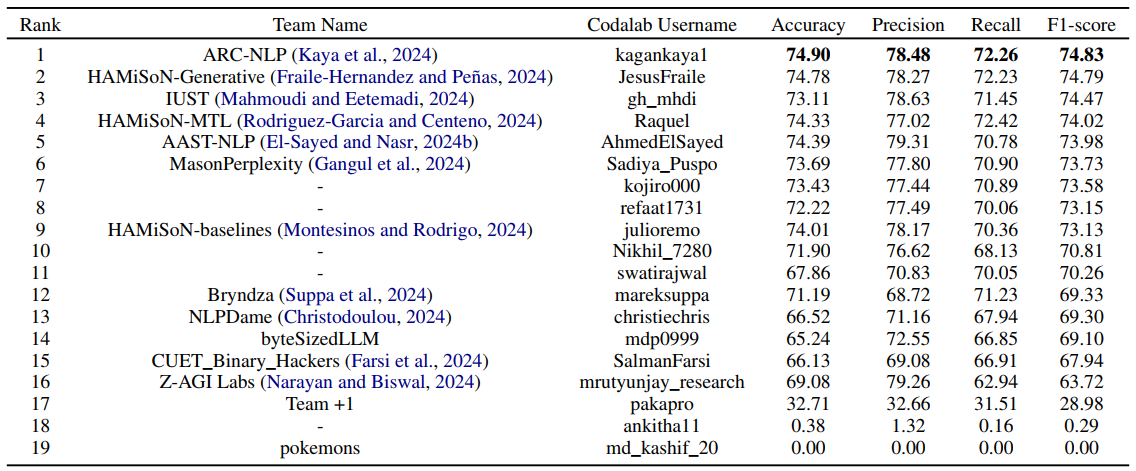
\includegraphics[width=1\linewidth]{images/Climate_Activism_result.PNG}}
	\end{figure}
 	\caption[نتایج رویداد
 	\lr{ClimateActivismStance}
 	برای زیر مسئله سوم (تشخیص موضع)]
 	{\label{climate_activism_result}  نتایج رویداد
 	\lr{ClimateActivismStance}
 	برای زیر مسئله سوم (تشخیص موضع)
 	\cite{thapa2024stance}
 }
 \end{table}

\section{مجموعه داده‌های مسئله تشخیص موضع}
با وجود اینکه تشخیص موضع، یک مسئله نوظهور و جدید است، اخیرا تلاش‌های قابل توجهی برای جمع آوری مجموعه داده در این حوزه انجام شده است. اغلب مجموعه دادە‌ها به صورت عمومی در دسترس تمام افراد قرار دارد. مجموعه دادە‌های جمع‌آوری‌شده معمولا از متن‌های مختلف از جمله توییت‌ها، پست‌ها در سایت‌های آنلاین، مقالات خبری و یا نظرات درباره خبرها جمع‌آوری شدە‌اند. 

مجوعه داده
\lr{Multi-Target}\cite{sobhani-etal-2017-dataset}
شامل توییت‌هایی در مورد چهار تن از نامزد‌های انتخابات ریاست جمهوری
آمریکا است. این افراد شامل دونالد ترامپ، هیلاری کلینتون، تد کروز و برنی سندرز می‌باشند. هر موضوع شامل دو تن از کاندیدا ریاست جمهوری می‌باشد (جدول
\ref{dataset-multitarget}). بنابراین برای هر موضوع دو برچسب موجود است (به ازای هر کاندید موضع توییت مشخص می‌شود). مجموعه داده شامل ۴۴۵۵ توییت که به صورت دستی برچسب زده شده است. این مجموعه داده، اولین مجموعه داده معرفی شده به صورت چند موضوعی
\lr{(Target-Multi)}
می‌باشد.
\begin{table}[ht]
	\centering
	\small
	\caption[توزیع نمونە ها در مجموعه داده
	\lr{Multi-Target}]{\label{dataset-multitarget} توزیع نمونە ها در مجموعه داده
		\lr{Multi-Target}\cite{sobhani-etal-2017-dataset}}
	
	\begin{figure}[H]
		\center{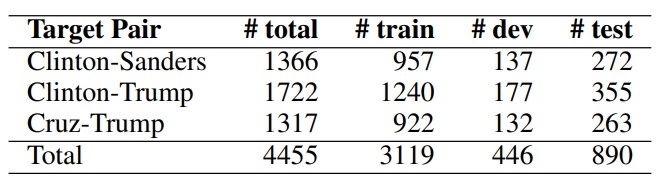
\includegraphics[width=0.5\linewidth]{images/Multi_target.jpg}}
	\end{figure}
	
\end{table}
مجموعه داده
\lr{WT-WT}\LTRfootnote{Will-They-Won’t-They}\cite{conforti-etal-2020-will}
جمع‌آوری شده به زبان انگلیسی شامل ۵۱۲۸۴ توییت می‌باشد. مجموعه داده جهت تشخیص موضع شایعه در بازارهای مالی جمع آوری شده است. توییت‌های جمع‌آوری شده درباره بحث‌های صورت گرفته در خصوص واگذاری یک شرکت به شرکت دیگر و یا تجمیع دو شرکت است.

مجموعه داده
\lr{X-Stance}\cite{vamvas2020xstance}
شامل 67000 داده در ارتباط با کاندیدا ریاست جمهوری سوییس به چهار زبان انگلیسی، آلمانی، فرانسوی و ایتالیایی می‌باشد. مجوعه داده
\lr{P-Stance}\cite{li-etal-2021-p}
شامل ۲۱۵۷۴ توییت به زبان انگلیسی درباره سه کاندید ریاست جمهوری آمریکا شامل دونالد ترامپ، جوبایدن و برنی سندز می‌باشد. مجموعه دادە‌های قبلی جمع آوری شده از توییتر، اغلب شامل دادە‌های بسیار کمی بودند. همین موضوع انگیزە ای برای جمع آوری مجموعه داده
 
\lr{P-Stance}
شد. مجموعه داده
\lr{VAST}\cite{Allaway2020Zero}
برای تشخیص موضع بدون داده آموزشی 
\LTRfootnote{Zero-Shot}
یا با داده آموزشی کم
\LTRfootnote{Few-Shot}
از نظرات موجود در تیویورک تایم جمع آوری شده است. این مجموعه داده شامل موضوعات متنوعی است. از هر موضوع تعداد داده کمی در مجموعه داده
موجود است. 

تا به اینجا معرفی مختصر بر تعدادی از مجوعه‌ داده‌های تشخیص موضع داشتیم. در ادامه به معرفی دقیق‌تر دو مجموعه داده \lr{SemEval-2016} و \lr{ClimaConvo} در این پژوهش می‌پردازیم.

\subsection{مجموعه داده
	\lr{SemEval-2016}
}

از معروف ترین مجموعه دادگان به زبان انگلیسی برای مسئله تشخیص موضع که در پژوهش های زیادی مورد استفاده قرار گرفته، مجموعه داده
 \lr{SemEval}
  است. این مجموعه داده برای اولین بار در رویداد
  \lr{SemEval2016}
برای دو زیر مسئله تشخیص موضع با نظارت و تشخیص موضع با نظارت ضعیف معرفی شد. این مجموعه داده از شش موضوع شامل انکار وجود خدا
\LTRfootnote{\lr{Atheism}}،
نگرانی از تغییرات آب و هوایی
\LTRfootnote{\lr{Climate Change is Concern}}،
جنبش فمینیسم
\LTRfootnote{\lr{Feminist Movement}}،
هیلاری کلینتون
\LTRfootnote{\lr{Hillary Clinton}}،
قانونی شدن سقط جنین
\LTRfootnote{\lr{Legalization of Abortion}}
و دونالد ترامپ
\LTRfootnote{\lr{Donald Trump}}
تشکیل شده است.

مجموعه دادگان
\lr{SemEval}
اولین مجموعه داده جمع‌آوری‌شده از پست‌های توییتر برای موضوع خاص
در مسئله تشخیص موضع است. این مجموعه داده علاوه بر برچسب تشخیص موضع، شامل برچسب تحلیل احساسات نیز می‌باشد. مجموعه داده توسط افراد و به صورت دستی، طبق پروتکل خاص برچسب گذاری شده است. چند نمونه از دادە‌های موجود در مجموعه داده در جدول~\ref{dataset-semeval} نشان داده شده است.


\begin{table}[ht]
	\centering
	\small
	\caption[چند نمونه از دادە‌های مجموعه داده
	\lr{SemEval}]{\label{dataset-semeval}  چند نمونه از دادە‌های مجموعه داده
		\lr{SemEval}\cite{mohammad-etal-2016-semeval}}
	
	\begin{figure}[H]
		\center{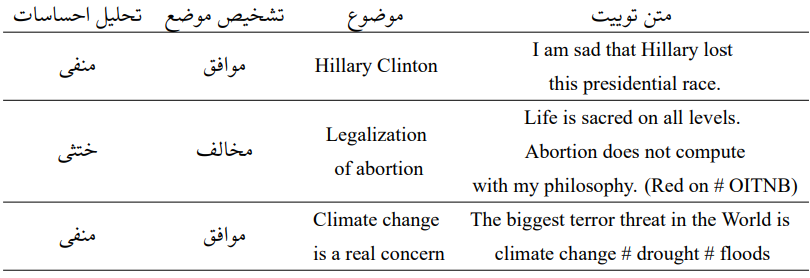
\includegraphics[width=0.9\linewidth]{images/semeval_example.PNG}}
	\end{figure}
	
\end{table}

برای جمع‌آوری مجموعه داده هشتک‌های خاصی در توییتر سرچ شدند. سپس تنها توییت‌هایی که در انتها آن‌ها هشتک وجود داشت نگه داشته و مابقی توییت‌ها حذف شدند. همچنین گاهی از روی هشتک موجود، می‌توان موضع را تشخیص داد. بنابراین هشتک‌های توییت‌ها نیز حذف شدند. برای جمع‌آوری دادە‌ها قوانین خاصی در نظر گرفته شد. به عنوان مثال اینکه (۱) توییت‌ها توسط مردم آمریکا قابل فهم باشد. (۲) برای
هر موضوع خاص از هر سه کلاس موافق، مخالف و بدون نظر داده به اندازه کافی وجود داشته باشد. (۳) مجموعه داده بهتر است شامل توییت‌هایی باشد که بدون اشاره مستقیم به هدف، موضع خود را نسبت به هدف بیان کند. (۴) مجموعه داده باید شامل دادە‌هایی باشد که هدف مورد نظر توییت با موضوع انتخابی توسط ما متفاوت باشد.
در نهایت مجموعه دادە ای شامل ۴۸۷۰ داده جمع آوری شد. توزیع نمونە ها بر اساس موضوعات در جدول
\ref{dataset-semeval-statistic}
قابل مشاهده است .


\begin{table}[ht]
	\centering
	\small
	\caption[چند نمونه از دادە‌های مجموعه داده
	\lr{ClimaConvo}]{\label{dataset-semeval-statistic}  توزیع نمونە‌ها در مجموعه داده
	\lr{SemEval}\cite{mohammad-etal-2016-semeval}}
	
	\begin{figure}[H]
		\center{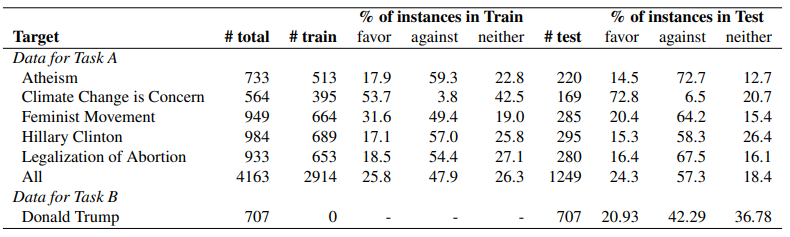
\includegraphics[width=0.9\linewidth]{images/SemEvalStatistic.PNG}}
	\end{figure}
	
\end{table}
\subsection{مجموعه داده
	\lr{ClimaConvo}
}\label{sec:datasetClimaConvo}
یکی از جدید‌ترین مجموعه داده‌های معرفی شده برای تشخیص موضع
\lr{ClimaConvo} \cite{shiwakoti2024analyzing}
می‌باشد. این مجموعه داده در رویداد
\lr{ClimateActivismStance}\cite{thapa2024stance}
معرفی و استفاده شده است. این مجموعه داده شامل حدود 15 هزار توییت در موضوع تغییرات اقلیمی می‌باشد. شش مسئله متفاوت پردازش زبان طبیعی بر روی این مجموعه داده تعریف شده است. داده‌های این مجموعه داده، مربوط به توییت‌های سال 2022 می‌باشد. برای جمع‌آوری مجموعه داده، توییت‌های شامل هشتک‌های مربوط به تغییرات اقلیمی جمع‌آوری شدند.  به عنوان مثال
\lr{\#climatecrisis, \#climatechange, \#ClimateEmergency, \#ClimateTalk, \#globalwarming}
نمونه‌ای از هشتگ‌های استفاده شده برای جمع‌آوری داده می‌باشد.
%\subsection{سایر مجموعه داده‌های تشخیص موضع}
\begin{table}[ht]
	\centering
	\small
	\caption[چند نمونه از دادە‌های مجموعه داده
	\lr{ClimaConvo}]{\label{dataset-climate-convo}  چند نمونه از دادە‌های مجموعه داده
		\lr{ClimaConvo}\cite{shiwakoti2024analyzing}}
	
	\begin{figure}[H]
		\center{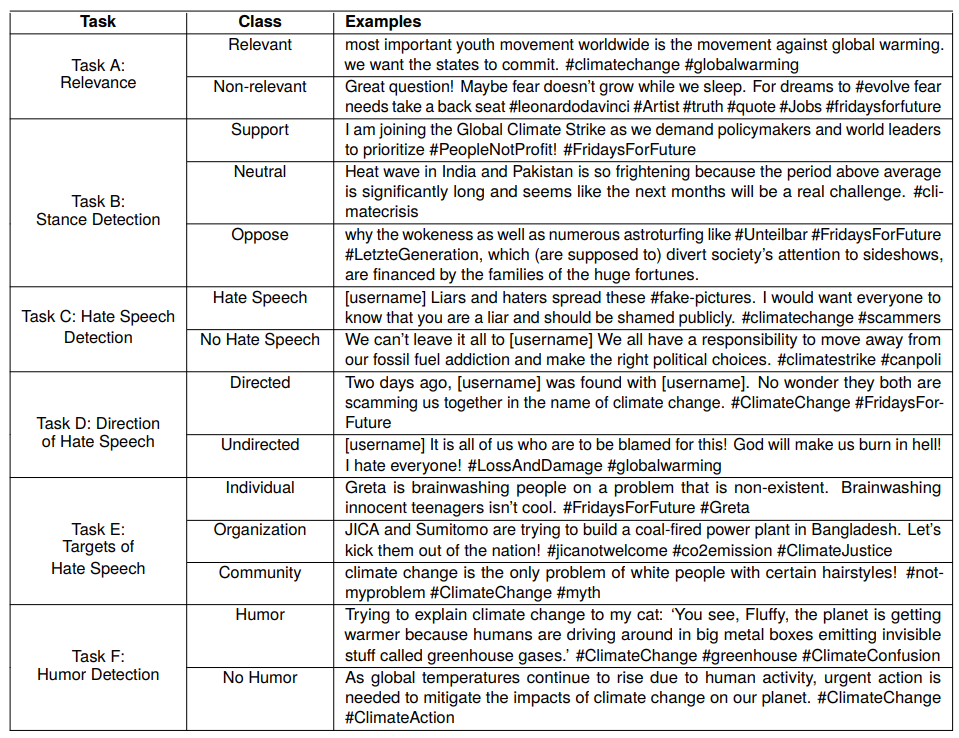
\includegraphics[width=1\linewidth]{images/ClimaConvo_Example.PNG}}
	\end{figure}
	
\end{table}


\section{پژوهش‌های انجام شده در مسئله تشخیص موضع}
همان‌طور که در بخش
\ref{sec:stance-detection-level}
اشاره شد، تشخیص موضع در سطوح متفاوتی تعریف می‌شود. شکل
\ref{stance_modeling_level}
شامل مروری جامع بر روش‌های ارائه شده در هر سطح می‌باشد. این شکل به صورت طبقه‌بندی شده ویژگی‌های مورد استفاده برای تشخیص موضع را نشان می‌دهد. در ادامه مروری بر روش‌های رده‌بندی در سطح محتوا
\LTRfootnote{Content}
 خواهیم داشت. رویکردهای ارائه شده را به دو دسته‌بندی کلی می‌توان تقسیم کرد. در ادامه پژوهش‌های هر بخش به طور مختصر معرفی خواهد شد.
\begin{figure}
	\center{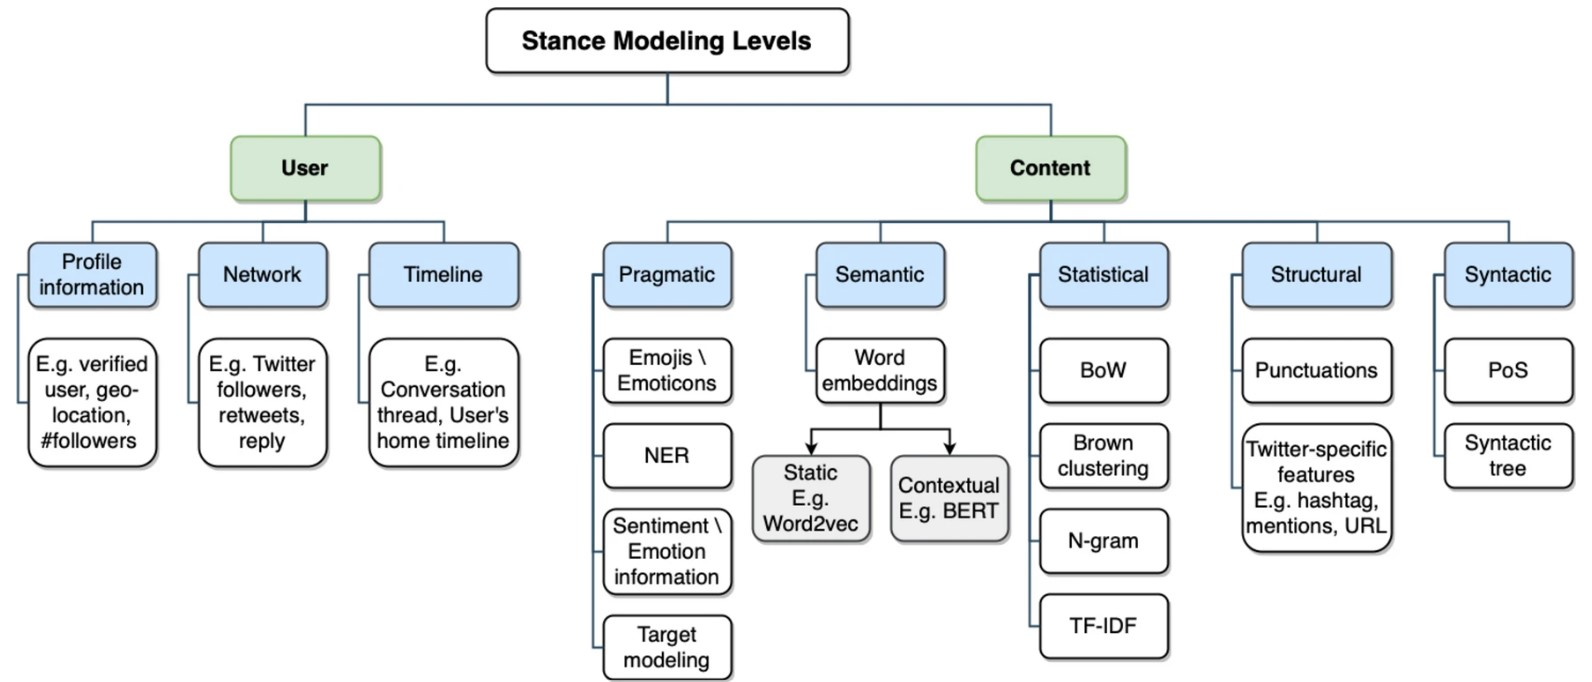
\includegraphics[width=1\linewidth]{images/stance_modeling_level.jpg}}
	\caption[مروری بر ویژگی‌های مورد استفاده در تشخیص موضع ]{مروری بر ویژگی‌های مورد استفاده در تشخیص موضع 
		\cite{Alturayeif2023} \label{stance_modeling_level}}
	
\end{figure}

\subsection[رویکردهای یادگیری ماشین مبتنی بر ویژگی]{رویکردهای یادگیری ماشین مبتنی بر ویژگی
	\LTRfootnote{\lr{Feature-Based Machine Learning Approaches}}}
%\begin{enumerate}
%	\item رویکردهای یادگیری ماشین مبتنی بر ویژگی
	%\LTRfootnote{Feature-Based Machine Learning Approaches}
	
	روش
	\lr{SVM}
	متداول‌ترین رویکرد یادگیری ماشین مبتنی بر ویژگی برای تشخیص موضع می‌باشد
	\cite{10.1145/3097286.3097288, 10.1145/3132169, mohammad-etal-2016-semeval, 10.1145/3269206.3271783, Sobhani2016DetectingSI}. 
این مدل در بیش از 40 پژوهش مورد استفاده قرار گرفته است. همچنین
	\lr{Logistic Regression}\cite{Kucher2020, 10.1007/978-3-030-14687-0_16}،
	\lr{naïve Bayes}
	و درخت تصمیم جز رده‌بند‌های متداول استفاده شده هستند. از دیگر الگوریتم‌های استفاده شده می‌توان به
	\lr{KNN}
	و 
	\lr{k-means	clustring}\cite{10.1007/978-3-319-66429-3-70}
	اشاره کرد.


مارتین و همکاران
\cite{tutek-etal-2016-takelab}
ترکیبی از چندین روش یادگیری را برای حل مسئله تشخیص موضع پیشنهاد می‌کنند. در این پژوهش از چهار مدل شامل 
\lr{SVM}، 
\lr{Random Forest}، 
\lr{Gradient Boosting} و 
\lr{Logistic Regression}
استفاده می‌شود. این الگوریتم برای ترکیب نتایج به دست آمده از چهار مدل نام برده شده،از الگوریتم ژنتیک استفاده می‌کند. ویژگی‌های واژگان به عنوان ورودی مدل برای ردە بندی انتخاب می‌شوند. این ویژگی‌ها شامل بازنمایی لغات،
\lr{n-gram}
در سطح کلمه و کاراکتر می‌باشد. همچنین تعدادی ویژگی مخصوص حل مسئله تشخیص موضع نیز تعریف کردند. این ویژگی‌ها شامل تعداد هشتگ‌ها، تعداد برخی کلمات خاص و یا غلط‌های املایی می‌باشد. این ویژگی‌ها به صورت دستی تعریف می‌شوند.


	مشیل و همکاران
	\cite{wojatzki-zesch-2016-ltl}،
	روش ردە بندی پشت سر هم
	\LTRfootnote{Stacked Classifications}
	را برای حل تشخیص موضع معرفی کردند. در واقع ردە بندی سه کلاسه در دو مرحله، با حل دو ردە بندی دو کلاسه انجام می‌شود. مرحله اول مشخص می‌کند آیا موضعی وجود دارد یا خیر. خروجی این مرحله دو بر چسب بدون موضع 
	\lr{(None)}
	یا با موضع مشخص
	\lr{(Against/Favor)}
است. سپس در صورت نیاز، در مرحله دوم برچسب نهایی از بین موافق یا مخالف انتخاب می‌شود. ردە بند استفاده شده در این روش، مدل
 SVM
 می‌باشد. واژگان موضع
 \LTRfootnote{Stance-lexicon Features}
  از مهم ترین ویژگی‌هایی است که برای ردە بندی به عنوان ورودی به مدل داده می‌شود.
  \begin{figure}
  	\center{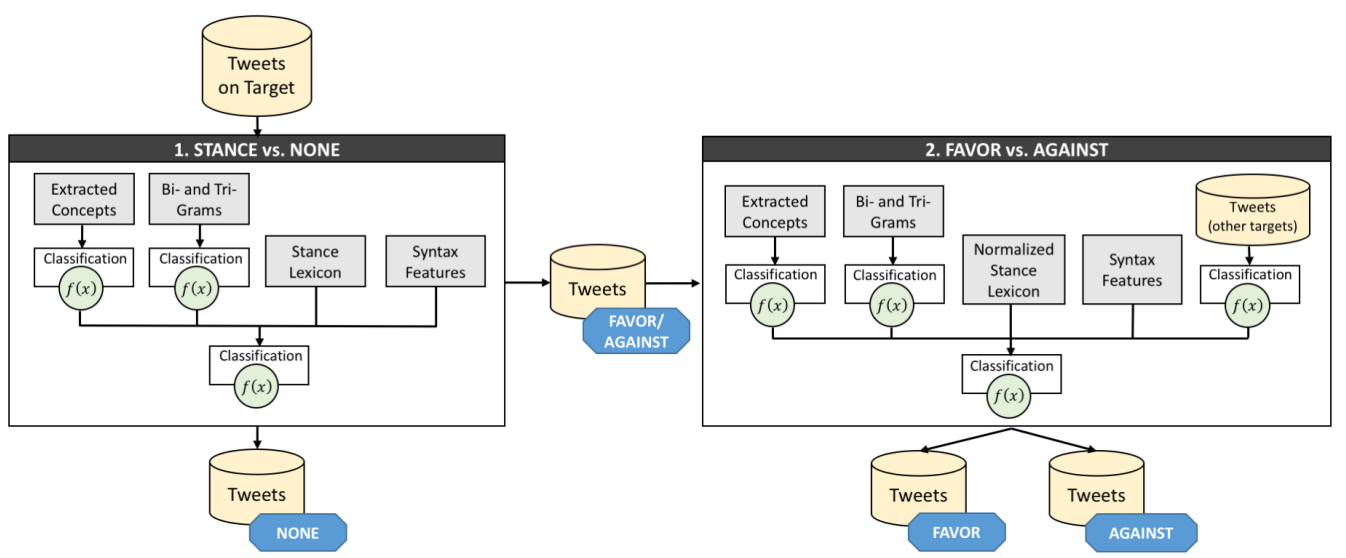
\includegraphics[width=1\linewidth]{images/StackedClassifier.PNG}}
  	\caption[معماری روش مبتنی بر 
  	\lr{Classifier Stacked}]{معماری روش مبتنی بر 
  		\lr{Classifier Stacked}
  		\cite{wojatzki-zesch-2016-ltl} \label{StackedClassifier}}
  	
  \end{figure}

\begin{table}[ht]
	\centering
	\small
	\caption[چند نمونه از پژوهش‌های مسئله تشخیص موضع]{\label{ML-Approach} چند نمونه از پژوهش‌های مسئله تشخیص موضع}
	
	\begin{tabular}{c c  c c c}
		
		پژوهش &  ویژگی & مدل & سال & مجموعه داده
		\\
		\hline
		\lr{ARC-NLP} \cite{thapa2024stance} &  
		\lr{CE \tablefootnote{contextualized embeddings}}
		& \lr{BERTweet}
		& 2023 & \lr{ClimaConvo}\\
		\hline
		\lr{HAMiSoN-G} \cite{thapa2024stance} &  
		\lr{prompt}
		& \lr{Llama}
		& 2023 & \lr{ClimaConvo}\\
		\hline
		\lr{Baseline} \cite{shiwakoti2024analyzing} &  
		\lr{CE}
		& \lr{ClimateBert}
		& 2023 & \lr{ClimaConvo}\\
		\hline
		\hline
    	\lr{PMINFM} \cite{10.1007/978-3-030-86365-4-22} &  
          \lr{CE, N-gram}
         &
         \begin{tabular}{@{}c@{}}
         	\lr{Ensemble model} \\ 
         	\lr{(RoBERTa+BiLSTM+attention)}\\
         \end{tabular}
         & 2021 & \lr{SE16-T6}\\
		\hline
         \lr{PE-HCN} \cite{zhao2020pretrained} &  
         \lr{CE, Topic modeling}
         &
          \begin{tabular}{@{}c@{}}
         	\lr{RoBERTa,} \\ 
         	\lr{Hierarchical capsule network}\\
         \end{tabular}
         & 2020 & \lr{SE16-T6}\\
		\hline
		\lr{HAN} \cite{sun-etal-2018-stance} &  
		\begin{tabular}{@{}c@{}}
			\lr{N-gram, POS, Structural} \\ 
			\lr{Sentiment lexicons}\\
		\end{tabular}
		
		& \lr{LSTM+attention}
		& 2018 & \lr{SE16-T6}\\
		\hline
		
		\cite{10.1007/978-3-030-36802-9-70} &  
		\begin{tabular}{@{}c@{}}
			\lr{SE\tablefootnote{static embeddings}, Topic modeling,} \\ 
			\lr{Sentiment labeling}\\
		\end{tabular}	
		& \lr{Multi-Task, Attention}
		& 2019 & \lr{SE16-T6}\\
		\hline
		\lr{MITRE} \cite{zarrella-marsh-2016-mitre} &  
		\lr{SE, Hashtag prediction}
		& \lr{LSTM}
		& 2016 & \lr{SE16-T6}\\
		\hline
		\hline
		\cite{Sobhani2016DetectingSI} &  
		\begin{tabular}{@{}c@{}}
			\lr{SE, Hashtag prediction} \\ 
			\lr{N-gram,Sentiment lexicons}\\
		\end{tabular}	
		& \lr{SVM}
		& 2016 & \lr{SE16-T6}\\
		\hline
		\cite{ebrahimi-etal-2016-joint} &  
		\begin{tabular}{@{}c@{}}
			\lr{N-gram, Sentiment lexicons} \\ 
			\lr{Topic modeling}\\
		\end{tabular}	
		& \lr{Maximum entropy}
		& 2016 & \lr{SE16-T6}\\
		\hline
		\lr{pkudblab} \cite{wei-etal-2016-pkudblab} &  
		\lr{SE}
		& \lr{CNN, voting scheme}
		& 2016 & \lr{SE16-T6}\\
	
		
		\hline
		\hline
		\lr{GPT3.5} \cite{zhang2022would} &  
		\lr{prompt}
		& \lr{GPT3.5}
		& 2022 & \lr{SE16-T6}\\
		\hline
		\lr{TPDG} \cite{10.1145/3442381.3449790} &  
		\begin{tabular}{@{}c@{}@{}}
			\lr{CE, Syntactical } \\ 
			\lr{dependency, Pragmatic}\\
			\lr{dependency graph}\\
		\end{tabular}
		&
		\lr{BiLSTM, GCN, attention}
		%, WT-WT
		& 2021 & \lr{SE16-T6}\\
		\hline
		\lr{SEKT} \cite{zhang-etal-2020-enhancing-cross} &  
		\begin{tabular}{@{}c@{}}
			\lr{SE, Semantic lexicons,} \\ 
			\lr{Knowledge graph}\\
		\end{tabular}
		&
		\begin{tabular}{@{}c@{}}
			\lr{GCN, BiLSTM+knowledge} \\ 
			\lr{-aware memory unit}\\
		\end{tabular}
		& 2020 & \lr{SE16-T6}\\
		\hline
		\lr{CrossNet} \cite{xu-etal-2018-cross} &  
		\lr{SE, CE, Target modeling}
		& \lr{Attention+MLP}
		& 2018 & \lr{SE16-T6}\\
		
		\hline
		\hline
		
		
	\end{tabular}
\end{table}

\iffalse
در ادامه متداول‌ترین ویژگی‌های استفاده شده در این رویکرد معرفی می‌شود. همچنین برخی ویژگی‌های در شکل
\ref{stance_modeling_level}
قابل مشاهده است.

\begin{itemize}
	\item ویژگی‌های لغوی مانند
	\lr{BOW}،
	\lr{n-gram}
	های کلمات و کاراکتر، هشتگ‌ها، کلمات نشان‌دهنده موضع، کلمات.
    \item بازنمایی برداری کلمات از جمله
	\lr{Word2Vec}،
	\lr{GloVe}.
\end{itemize}  
\fi  

\subsection[رویکردهای یادگیری عمیق]{رویکردهای یادگیری عمیق
	\LTRfootnote{\lr{Deep Learning Approaches}}}
	%\item رویکردهای یادگیری عمیق
	%\LTRfootnote{رویکردهای یادگیری عمیق}
	
	شبکه‌های عمیق در تعداد قابل توجهی از مطالعات در تشخیص موضع استفاده شدە اند.
	 \lr{RNN}
	 	  ها و انواع توسعه یافته آن 
	 \lr{(GRU ,LSTM)}	   
و شبکە‌های عصبی پیچشی
\lr{CNN}
 ها از جمله شبکە‌های عمیق استفاده شده	هستند. از میان روش‌های مطرح شده، مدل LSTM متداول ترین رویکرد استفاده شده برای تشخیص موضع
	می‌باشد. در ادامه به بررسی و معرفی برخی رویکردهای معروف پرداخته می‌شود. 
	
	برخی از ویژگی‌های متداول مورد استفاده در روش‌های یادگیری عمیق مرتبط، بازنمایی کلمات
	\lr{Word2vec}
	و
	\lr{GloVe}
	می‌باشد.
	
	در بسیاری از مطالعات اخیر از یک مکانیزم توجه استفاده شده تا عملکرد نهایی را بهبود بخشد
	\cite{10.1007/978-3-319-68783-4-2, 8489665}.
	
	مدل
	\lr{BiCond}\LTRfootnote{Bidirectional Conditional LSTM}
	توسط ایزابل و همکاران
	\cite{augenstein-etal-2016-stance}
	برای تشخیص موضع با نظارت ضعیف معرفی شده است. این روش از دو شبکه 
	\lr{BiLSTM}
	برای حل تشخیص موضع استفاده می‌کند. این دو شبکه به نحوی به یکدیگر وابسته هستند. اولین
	\lr{BiLSTM}
	وظیفه تولید بازنمایی از موضوع را به عهده دارد. دومین
	  \lr{BiLSTM}
	  نیز بازنمایی از متن توییت تولید می‌کند. نکته مهم در معماری
	  \lr{BiCond}
این است که آخرین مقادیر وزن
\lr{BiLSTM}
که موضوع را به عنوان ورودی گرفته، مقادیر اولیه
  \lr{BiLSTM}
ای است که در ادامه متن را به عنوان ورودی می‌گیرد. این وابستگی در
جهت برعکس متن اصلی نیز برقرار است. به همین دلیل است مدل شرطی نام گرفته است. این وابستگی بین موضوع و متن توییت در معماری به وضوح در شکل
\ref{bicond}
(با خط چین قرمز) قابل مشاهده است. این معماری با توجه به وابستگی که بین موضوع و متن توییت ایجاد می‌کند، عملکرد بهتری در تشخیص موضع
با نظارت ضعیف از خود نشان داده است. همچنین نتایج خوبی در تشخیص موضع برای موضوعاتی که در زمان آموزش ندیده نیز به دست آورده است.

\begin{figure}
	\center{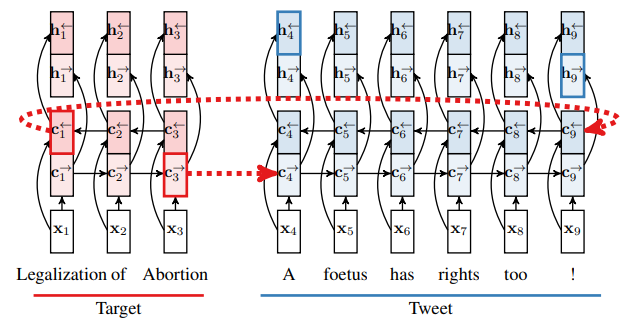
\includegraphics[width=0.8\linewidth]{images/BiCond.PNG}}
	
	\caption[معماری مدل
	\lr{BiCond}]{معماری مدل
	\lr{BiCond}\cite{augenstein-etal-2016-stance}}
	\label{bicond}
\end{figure}

مدل
\lr{PNEM}\cite{siddiqua-etal-2019-tweet}
یک روش ترکیبی برای تشخیص موضع است. در این مدل از
 \lr{CNN، LSTM}
و مکانیزم توجه استفاده شده است. ابتدا با استفاده از چندین کرنل در شبکه CNN ویژگی‌های سطح بالا از بردار متن و موضوع استخراج می‌شود. در ادامه بردار بازنمایی به دست آمده به عنوان ورودی به 
\lr{DC-BiLSTM}\LTRfootnote{Densely Connected BiLSTM}
و
\lr{NLSTMs}\LTRfootnote{Nested LSTMs}
داده می‌شود. سپس دو بردار بازنمایی تولید شده پس از عبور از مکانیزم توجه برای ردە‌بندی به شبکه کاملا متصل وارد می‌شوند. در نهایت با استفاده از بردار بازنمایی نهایی کلاس برنده مشخص می‌شود.

\begin{figure}
	\center{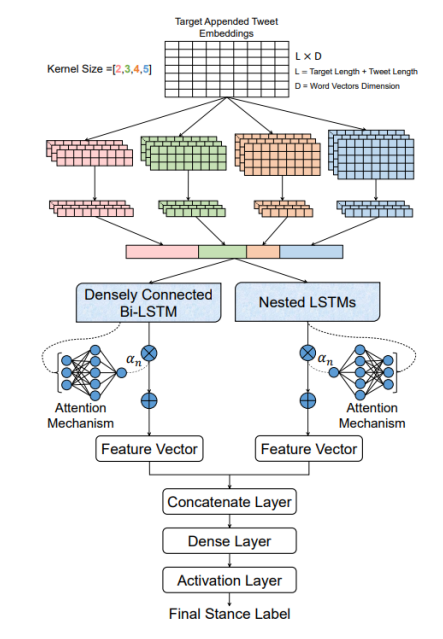
\includegraphics[width=0.4\linewidth]{images/PNEM.PNG}}
	
	\caption[معماری مدل
	\lr{PNEM}]{معماری مدل
		\lr{PNEM}\cite{siddiqua-etal-2019-tweet}}
	\label{PNEM}
\end{figure}

\subsection[مدل‌های از قبل آموزش دیده]{مدل‌های از قبل آموزش دیده}
	
	
	در سال‌های اخیر مدل‌های از پیش آموزش دیده در حوزه پردازش زبان طبیعی تعریف شده است. این مدل‌ها مبتنی بر ترنسفورمر هستند و به دلیل آموزش بر روی حجم بسیار زیادی از دادە‌ها، قابلیت بازنمایی از کلمات
دارند. 

مدل 
\lr{TweetEval}\cite{barbieri-etal-2020-tweeteval}
یک ارزیابی مبنایی 
\LTRfootnote{text}{Evaluation Benchmark}
برای شبکه اجتماعی توییتر تعریف می‌کند. 
\lr{TweetEval}
 بر روی ۷ مجموعه داده جمع آوری شده از توییتر ارزیابی شده است. بهترین نتایج با رویکرد استفاده از وزن‌های از پیش تعیین شده
\lr{RoBERTa}  
و آموزش مجدد با دادە های توییتر به دست می‌آید.

مدل
\lr{TimeLMs}\cite{loureiro-etal-2022-timelms}
 یک مدل زبانی تعریف شده بر شبکه اجتماعی توییتر است. مشابه با
\lr{TweetEval}
مدل \lr{TimeLMs} نیز از \lr{RoBERTa} استفاده می‌کند. نحوه آموزش مدل نیز مشابه با روش انتخاب شده در
\lr{TweetEval}
 است. نکته جدیدی که در این پژوهش مدل نظر قرار گرفته این است که با توجه به تغییراتی که به صورت مداوم در نحوه نگارش در شبکه‌‌های اجتماعی رخ می‌دهد، نیاز است مدل به صورت ادامه دار آموزش ببیند. این مدل بازە‌های چهار ماهه را برای این کار انتخاب کرده است. به این صورت که هر چهار ماه یه بار مدل پیشین بر روی دادە‌هایی که اخیرا از شبکه‌های اجتماعی استخراج شده آموزش ببیند. بدین ترتیب مدل زبانی همواره به روز می‌ماند.

یکی دیگر از مدل‌های زبانی استفاده شده در تشخیص موضع 
\lr{MeLT}\cite{matero-etal-2021-melt-message}
می‌باشد. روش‌های قبلی مدل زبانی را بر روی یک پیام کاربر و با حذف توکن‌های آن آموزش می‌دادند. گاهی تنها با بررسی یک پیام کاربر نمی‌توان موضع پیام نسبت به موضوع خاصی را تشخیص داد. اما زمانی که سایر متن‌های نوشته شده از کاربر بررسی می‌شود، موضع پیام قبلی که تشخیص آن سخت بود نیز میسر می‌شود. بنابراین این ایده مطرح شد که پیام‌های کاربر به صورت پشت سر هم دیده شود. به این منظور چهل پیام اخیر هر کاربر انتخاب می‌شود. و به کمک مدل زبانی از هر پیام یک بردار بازنمایی تولید می‌شود. در ادامه همان روش آموزش مدل های زبانی استفاده می‌شود. با این تفاوت که این بار به جای حذف یک توکن متن، بردار بازنمایی یک پیام کاربر
حذف می‌شود (شکل
\ref{MeLT})
و مدل زبانی آموزش می‌بیند تا این بردار را مجددا تولید کند.
\begin{figure}[H]
	\center{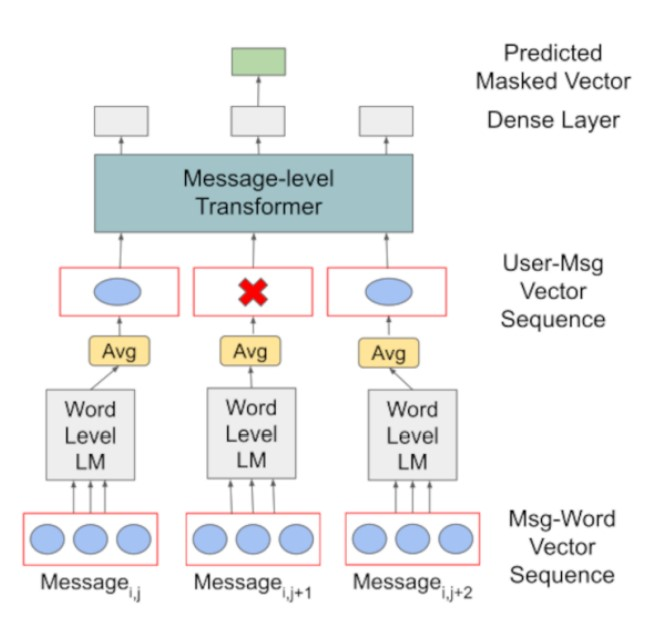
\includegraphics[width=0.6\linewidth]{images/MeLT.jpg}}
	\caption[معماری مدل
	\lr{MeLT}]{معماری مدل
		\lr{MeLT}\cite{matero-etal-2021-melt-message}}
	\label{MeLT}
\end{figure}

در پژوهش 
\cite{zhang2022would}
ژنگ و همکاران با 
\lr{ChatGPT}
و پیشنهاد پرامپت، مسئله تشخیص موضع را حل کردند. شکل
\ref{GPT_Stance}
پرامپت ارائه شده توسط این مقاله برای تعامل با 
\lr{ChatGPT}
نشان می‌دهد.
\begin{figure}[H]
	\center{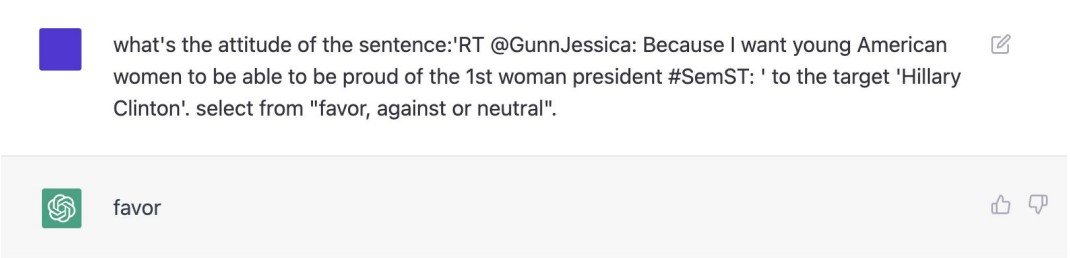
\includegraphics[width=0.8\linewidth]{images/GPT_Stance.PNG}}
	
	\caption[معماری مدل
	\lr{BiCond}]{پرامپت پیشنهادی پژوهش
		\cite{zhang2022would}}
	\label{GPT_Stance}
\end{figure}


	%\LTRfootnote{Ensemble Learning Approaches}
	
	%\item رویکرد یادگیری مجمع
	%\LTRfootnote{Ensemble Learning Approaches}
	%\item رویکرد یادگیری انتفالی
	%\LTRfootnote{Transfer Learning Approaches}
%\end{enumerate}

\iffalse


\subsection{رویکردهای مبتنی بر یادگیری با داده‌های آموزشی کم یا بدون داده آموزشی}
\lr{Zhang et al.21 employed ChatGPT for stance detection, which includes support and opposition. They used ChatGPT to classify the political stance of tweets in the SemEval-2016 and P-Stance datasets. SemEval-2016 contains 4870 English tweets, and they selected tweets with the most commonly occurring FM, LA, and HC political labels for stance classification. The P-Stance dataset has 21,574 English tweets, and they classified the stance of tweets towards Trump, Biden, and Bernie. The final results showed that on the SemEval-2016 dataset, ChatGPT achieved F1-m scores of 68.4, 58.2, and 79.5 for the FM, LA, and HC political labels, and F1-avg scores of 72.6, 59.3, and 78.0, respectively. On the P-Stance dataset, ChatGPT achieved F1-m scores of 82.8, 82.3, and 79.4 for the Trump, Biden, and Bernie political figures, and F1-avg scores of 83.2, 82.0, and 79.4, respectively.}
\fi
\section{معیار ارزیابی مسئله تشخیص موضع}
معیارهای
\lr{Precision}، 
\lr{Recall }
و 
\lr{F-Score}
معمولا در مسائل بازیابی اطلاعات
\LTRfootnote{\lr{Information Retrieval}}
و استخراج اطلاعات
\LTRfootnote{\lr{Information Extraction}}
مورد استفاده قرار می‌گیرد. معیار
\lr{F-Score}
 با وزن‌دهی بر دو معیار
 \lr{Precision}
 و
 \lr{Recall}
  محاسبه می‌شود. معیار ارزیابی
  \lr{F-Score}
همچنین در مسئله تشخیص موضع با سه کلاس نیز مورد قرار می‌گیرد. پرکاربردترین نسخه
\lr{F-Score}
 به صورت میانگین کلان
 \LTRfootnote{\lr{Macro Average}}
است که صورت زیر محاسبه می‌شود.
 \begin{equation}
	Accuracy = \frac{TP+TN}{TP+TN+FP+FN}
\end{equation}
 
\begin{equation}
 	Precision = \frac{TP}{TP+FP}
\end{equation}

\begin{equation}
	Recall = \frac{TP}{TP+FN}
\end{equation}

\begin{equation}
	F1 = \frac{2*Precision*Recall}{Precision+Recall} = \frac{2*TP}{2*TP+FP+FN}
\end{equation}


